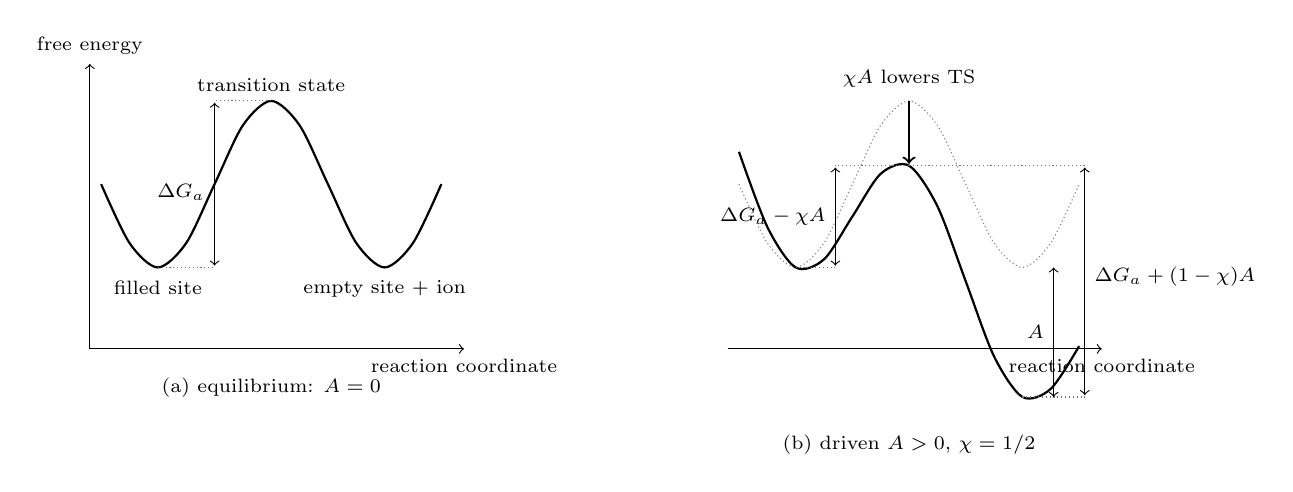
\begin{tikzpicture}[x=0.72cm,y=2.35cm]
\draw[->] (-0.2,-0.34) -- (6.4,-0.34) node[below,font=\scriptsize] {reaction coordinate};
\draw[->] (-0.2,-0.34) -- (-0.2,1.20) node[above,font=\scriptsize] {free energy};
\draw[thick] plot[smooth] coordinates {(0.0,0.550) (0.5,0.232) (1.0,0.100) (1.5,0.232) (2.0,0.550) (2.5,0.868) (3.0,1.000) (3.5,0.868) (4.0,0.550) (4.5,0.232) (5.0,0.100) (5.5,0.232) (6.0,0.550)};
\node[below,font=\scriptsize] at (1,0.08) {filled site};
\node[below,font=\scriptsize] at (5,0.08) {empty site + ion};
\node[above,font=\scriptsize] at (3,1.0) {transition state};
\draw[densely dotted,black!55] (1,0.1) -- (2.0,0.1);
\draw[densely dotted,black!55] (3,1.0) -- (2.0,1.0);
\draw[<->] (2.0,0.11) -- (2.0,0.99) node[pos=0.45,left,font=\scriptsize] {$\Delta G_a$};
\node[font=\scriptsize] at (3,-0.55) {(a) equilibrium: $A=0$};
\begin{scope}[xshift=8.1cm]
\draw[->] (-0.2,-0.34) -- (6.4,-0.34) node[below,font=\scriptsize] {reaction coordinate};
\draw[densely dotted,thin,black!50] plot[smooth] coordinates {(0.0,0.550) (0.5,0.232) (1.0,0.100) (1.5,0.232) (2.0,0.550) (2.5,0.868) (3.0,1.000) (3.5,0.868) (4.0,0.550) (4.5,0.232) (5.0,0.100) (5.5,0.232) (6.0,0.550)};
\draw[thick] plot[smooth] coordinates {(0.0,0.725) (0.5,0.319) (1.0,0.100) (1.5,0.144) (2.0,0.375) (2.5,0.606) (3.0,0.650) (3.5,0.431) (4.0,0.025) (4.5,-0.381) (5.0,-0.600) (5.5,-0.556) (6.0,-0.325)};
\draw[->,thick] (3.0,1.00) -- (3.0,0.66);
\node[above,font=\scriptsize] at (3.0,1.02) {$\chi A$ lowers TS};
\draw[densely dotted,black!55] (1.0,0.1) -- (1.70,0.1);
\draw[densely dotted,black!55] (3.0,0.65) -- (1.70,0.65);
\draw[<->] (1.70,0.11) -- (1.70,0.64) node[pos=0.50,left,font=\scriptsize] {$\Delta G_a-\chi A$};
\draw[densely dotted,black!55] (5.0,-0.60) -- (6.10,-0.60);
\draw[densely dotted,black!55] (3.0,0.65) -- (6.10,0.65);
\draw[<->] (6.10,-0.59) -- (6.10,0.64) node[pos=0.52,right,font=\scriptsize] {$\Delta G_a+(1-\chi)A$};
\draw[<->] (5.55,0.10) -- (5.55,-0.60) node[pos=0.50,left,font=\scriptsize] {$A$};
\node[font=\scriptsize] at (3,-0.86) {(b) driven $A>0$, $\chi=1/2$};
\end{scope}
\end{tikzpicture}
\caption{활성화 장벽 그림. (a) 평형에서는 두 골짜기 높이가 같고 속도는 Eyring 식을 따른다. (b) 구동력 $\mathcal A_j$가 도착 골짜기를 내리면 정방향 장벽은 $\Delta G_a-\chi\mathcal A$, 역방향 장벽은 $\Delta G_a+(1-\chi)\mathcal A$로 비대칭 이동한다(식~\eqref{eq:bv}; 속도비는 식~\eqref{eq:db} detailed balance). 기존 두 패널 구도를 보존하되 전이상태 하강량과 역장벽 상승량을 함께 표시했다. 좌표는 \code{T4\_calc.py}의 cosine-squared 장벽과 선형 affinity tilt 평가값이다.}
\label{fig:barrier}
